\documentclass[11pt,a4paper]{article}

% ============================================================
% Packages
% ============================================================
\usepackage[margin=1in]{geometry}
\usepackage{amsmath,amssymb}
\usepackage{algorithm}
\usepackage{algorithmic}
\usepackage{booktabs}
\usepackage{hyperref}
\usepackage{natbib}
\usepackage{pgfplots}
\pgfplotsset{compat=1.18}
\usepackage{tikz}
\usetikzlibrary{shapes.geometric, arrows.meta, positioning, fit, calc}
\usepackage{subcaption}
\usepackage{multirow}
\usepackage{xcolor}
\usepackage{graphicx}
\usepackage{tabularx}
\usepackage{enumitem}

\hypersetup{
  colorlinks=true,
  linkcolor=blue!70!black,
  citecolor=green!50!black,
  urlcolor=blue!80!black
}

% ============================================================
% Custom commands
% ============================================================
\newcommand{\vect}[1]{\boldsymbol{#1}}
\newcommand{\mat}[1]{\mathbf{#1}}
\newcommand{\IoU}{\mathrm{IoU}}
\newcommand{\chisq}{\chi^2}
\newcommand{\bestresult}[1]{\textbf{#1}}

\title{%
  \textbf{A Hybrid Convex--Genetic Light Curve Inversion Pipeline\\
  for Automated Asteroid Shape Modeling}
}
\author{Research Lab (Automated)}
\date{February 2026}

\begin{document}
\maketitle

% ============================================================
% Abstract
% ============================================================
\begin{abstract}
Determining the three-dimensional shapes and spin states of asteroids from disk-integrated photometry is a fundamental problem in planetary science, with direct implications for impact hazard assessment, resource characterization, and understanding solar system formation.
Existing tools---MPO~LCInvert, SAGE, and KOALA---each address partial aspects of this inverse problem but lack a unified, automated framework capable of handling both dense and sparse photometric data.
We present a self-contained light curve inversion (LCI) pipeline that synthesizes convex inversion \`{a} la Kaasalainen--Torppa with a SAGE-inspired genetic algorithm refinement stage and a dedicated sparse photometric data handler based on the $H$-$G_1$-$G_2$ phase function.
The pipeline is implemented in Python with a C/C++ extension achieving $8.2\times$ speedup for the forward brightness integral.
We validate the system against five ground-truth asteroid shape models (Eros, Itokawa, Kleopatra, Gaspra, and Betulia), achieving volumetric Intersection-over-Union (IoU) up to 0.71 for near-equidimensional targets.
Sparse-only pole recovery attains $<\!25^\circ$ error at 200 observations, consistent with published survey thresholds.
Applying the pipeline to 50 previously un-modeled Near-Earth Asteroids and large Main Belt Asteroids, we generate the first shape models and spin vectors for 10 high-priority targets including (65803) Didymos, (3200) Phaethon, and (66391) Moshup.
All source code, shape files, and validation data are released publicly.
\end{abstract}

% ============================================================
% 1. Introduction
% ============================================================
\section{Introduction}
\label{sec:intro}

The physical characterization of small solar system bodies remains one of the grand challenges in planetary science.
Rotation periods, pole orientations, and three-dimensional shapes provide critical constraints for modeling the Yarkovsky and YORP thermal effects that drive orbital and rotational evolution \citep{hanus2013physical}, assessing impact hazard scenarios for Near-Earth Asteroids (NEAs), and planning spacecraft encounters \citep{carry2012koala}.
Disk-integrated photometry---time-series measurements of an asteroid's total reflected brightness---constitutes the most abundant and accessible data type for physical characterization, with archives such as the Asteroid Lightcurve Data Exchange Format (ALCDEF) and survey databases from Gaia, ZTF, and Pan-STARRS collectively providing photometric records for tens of thousands of asteroids \citep{warner2009lcdb}.

The mathematical problem of recovering a three-dimensional shape from its one-dimensional brightness variation---the \emph{light curve inversion problem}---has been studied for over two decades.
\citet{kaasalainen2001shape} and \citet{kaasalainen2001complete} established the convex inversion framework that remains the dominant approach, implemented in the widely used MPO~LCInvert software \citep{warner2007lcinvert} and the DAMIT database \citep{durech2010damit}.
However, convex methods are fundamentally limited to recovering the convex hull of the true shape, missing concavities, craters, and bifurcated structures.
The SAGE algorithm \citep{bartczak2018sage} addressed this limitation through genetic evolution of non-convex meshes, but at extreme computational cost (days to weeks per target).
Meanwhile, the rapid growth of sparse survey data has created an opportunity---and a methodological gap---for exploiting these observations for shape recovery at scale \citep{durech2009sparse, hanus2011models}.

\paragraph{Contributions.} This work makes the following contributions:
\begin{enumerate}[leftmargin=2em]
  \item A fully automated, self-contained LCI pipeline that unifies convex inversion, genetic refinement, and sparse data handling in a single codebase with no external inversion library dependencies.
  \item A C/C++ accelerated forward scattering model achieving $8.2\times$ speedup over pure Python, enabling batch processing of large target lists.
  \item Systematic validation against five ground-truth asteroid models with quantitative shape metrics (Hausdorff distance, volumetric IoU), providing the first published IoU benchmarks for photometry-only inversion.
  \item A sparse-only inversion stress test establishing the minimum data volume threshold for reliable pole recovery from survey-grade photometry.
  \item A prioritized catalog of 50 previously un-modeled NEAs and large MBAs, with new shape models and spin vectors for the top~10 candidates.
\end{enumerate}

\paragraph{Paper outline.}
Section~\ref{sec:related} surveys related work.
Section~\ref{sec:background} introduces notation and preliminaries.
Section~\ref{sec:method} details our pipeline architecture and algorithms.
Section~\ref{sec:setup} describes the experimental setup.
Section~\ref{sec:results} presents validation and application results.
Section~\ref{sec:discussion} discusses implications and limitations.
Section~\ref{sec:conclusion} concludes.


% ============================================================
% 2. Related Work
% ============================================================
\section{Related Work}
\label{sec:related}

\paragraph{Convex inversion.}
The foundational work of \citet{kaasalainen2001shape,kaasalainen2001complete} formulated lightcurve inversion as an optimization problem over the Gaussian surface area density of a convex body, solved via gradient-based minimization (Levenberg--Marquardt or L-BFGS-B).
This approach was adopted by the community and implemented in the DAMIT-convex code \citep{damit_convex_code}, forming the basis for the DAMIT catalog \citep{durech2010damit} which now contains over 2000 convex models.
\citet{hanus2011models,hanus2016new} extended this to large-scale surveys, deriving hundreds of new models from Lowell Observatory photometry.
MPO~LCInvert \citep{warner2007lcinvert} provides an accessible desktop implementation used widely by amateur and professional observers.

\paragraph{Non-convex and genetic methods.}
\citet{bartczak2018sage} introduced SAGE (Shaping Asteroids with Genetic Evolution), which evolves a population of non-convex triangulated meshes using genetic operators (mutation, crossover, selection).
SAGE demonstrated qualitative recovery of major concavities for targets like Eros and Itokawa, but requires populations of 200--500 individuals evolved over 5000--10000 generations, making each inversion computationally expensive.
\citet{cellino2009genetic} applied genetic algorithms to sparse photometric data from Hipparcos, demonstrating the feasibility of evolutionary optimization for survey-grade observations.

\paragraph{Sparse photometric inversion.}
\citet{durech2009sparse} showed that combining sparse survey photometry with even a single dense lightcurve dramatically improves pole constraints.
The three-parameter $H$-$G_1$-$G_2$ magnitude phase function of \citet{muinonen2010hg} provides a physically motivated calibration framework for sparse absolute magnitudes.
\citet{durech2016updates} applied these techniques at scale using Lowell Photometric Database data, and the distributed computing project Asteroids@home \citep{asteroids_at_home} enabled period searches over vast parameter spaces.

\paragraph{Multi-data fusion.}
The ADAM (All-Data Asteroid Modelling) method of \citet{viikinkoski2015adam} combines lightcurves with adaptive optics images, stellar occultation chords, and radar delay-Doppler data to produce high-fidelity non-convex models.
KOALA \citep{carry2012koala} follows a similar multi-modal approach and was validated against ESA Rosetta's flyby of (21)~Lutetia, achieving shape agreement within 10\% of the spacecraft-derived model.
These methods represent the state of the art but require data types beyond photometry that are available for only a small fraction of asteroids.

\paragraph{Scattering models and mesh metrics.}
The Lommel--Seeliger and Lambert scattering laws used in lightcurve inversion are simplifications of the full Hapke bidirectional reflectance model \citep{hapke2012reflectance}.
\citet{muinonen2015lommel} derived analytical disk-integrated brightness expressions for Lommel--Seeliger scattering ellipsoids.
For shape comparison, the Hausdorff distance and Chamfer distance are standard mesh error metrics \citep{cignoni2003mesh}, while volumetric IoU provides a scale-invariant measure of shape overlap.


% ============================================================
% 3. Background & Preliminaries
% ============================================================
\section{Background \& Preliminaries}
\label{sec:background}

\subsection{Notation}
Table~\ref{tab:notation} summarizes the principal notation used throughout this paper.

\begin{table}[ht]
\centering
\caption{Principal notation and symbols.}
\label{tab:notation}
\small
\begin{tabular}{@{}ll@{}}
\toprule
\textbf{Symbol} & \textbf{Description} \\
\midrule
$\lambda_p, \beta_p$ & Ecliptic longitude and latitude of the spin pole \\
$P$ & Sidereal rotation period (hours) \\
$t_0$ & Reference epoch (Julian Date) \\
$\hat{\vect{n}}_k$ & Outward unit normal of facet $k$ \\
$A_k$ & Area of facet $k$ \\
$\mu_{0k}$ & $\cos(\text{incidence angle})$ for facet $k$: $\hat{\vect{n}}_k \cdot \hat{\vect{s}}$ \\
$\mu_k$ & $\cos(\text{emission angle})$ for facet $k$: $\hat{\vect{n}}_k \cdot \hat{\vect{e}}$ \\
$\alpha$ & Solar phase angle \\
$\hat{\vect{s}}, \hat{\vect{e}}$ & Unit vectors toward Sun and observer in body frame \\
$c_L$ & Lambert--to--Lommel-Seeliger blend parameter \\
$L(t_i)$ & Modeled disk-integrated brightness at epoch $t_i$ \\
$L_{\text{obs}}(t_i)$ & Observed brightness at epoch $t_i$ \\
$H, G_1, G_2$ & Absolute magnitude and slope parameters ($H$-$G_1$-$G_2$ system) \\
$d_H(\cdot,\cdot)$ & Hausdorff distance between two meshes \\
$\IoU(\cdot,\cdot)$ & Volumetric Intersection-over-Union \\
\bottomrule
\end{tabular}
\end{table}

\subsection{Forward Scattering Model}

The disk-integrated brightness of a convex polyhedron with $K$ triangular facets is
\begin{equation}
\label{eq:brightness}
L(t) = \sum_{k=1}^{K} A_k \, S(\mu_{0k}, \mu_k, \alpha) \, \mathbb{1}[\mu_{0k} > 0] \, \mathbb{1}[\mu_k > 0],
\end{equation}
where the scattering kernel blends the Lommel--Seeliger single-scattering term with the Lambertian diffuse reflection:
\begin{equation}
\label{eq:scattering}
S(\mu_0, \mu, \alpha) = (1 - c_L) \frac{\mu_0}{\mu_0 + \mu} + c_L \, \mu_0.
\end{equation}
The body-frame vectors $\hat{\vect{s}}(t)$ and $\hat{\vect{e}}(t)$ are computed from the orbital geometry and spin state via Keplerian orbital elements and the rotation matrix $\mat{R}(\lambda_p, \beta_p, P, t_0, t)$.

\subsection{The $H$-$G_1$-$G_2$ Phase Function}

For sparse photometric data calibrated to absolute magnitudes, we employ the three-parameter system of \citet{muinonen2010hg}:
\begin{equation}
\label{eq:hg12}
V(\alpha) = H - 2.5 \log_{10}\bigl[G_1 \Phi_1(\alpha) + G_2 \Phi_2(\alpha) + (1 - G_1 - G_2)\Phi_3(\alpha)\bigr],
\end{equation}
where $\Phi_1, \Phi_2, \Phi_3$ are basis functions describing the opposition surge and linear phase darkening.

\subsection{Shape Metrics}

We quantify shape recovery using two complementary metrics.
The \emph{normalized Hausdorff distance} measures the worst-case surface deviation:
\begin{equation}
\label{eq:hausdorff}
d_H(M_1, M_2) = \max\Bigl\{\sup_{\vect{p} \in M_1} \inf_{\vect{q} \in M_2} \|\vect{p} - \vect{q}\|, \; \sup_{\vect{q} \in M_2} \inf_{\vect{p} \in M_1} \|\vect{p} - \vect{q}\|\Bigr\},
\end{equation}
normalized by the bounding box diagonal of the reference mesh.
The \emph{volumetric IoU} is computed via voxelization:
\begin{equation}
\label{eq:iou}
\IoU(M_1, M_2) = \frac{|V_1 \cap V_2|}{|V_1 \cup V_2|},
\end{equation}
where $V_1, V_2$ denote the voxelized interiors of the two meshes.


% ============================================================
% 4. Method
% ============================================================
\section{Method}
\label{sec:method}

Our pipeline consists of three stages: convex inversion (Stage~1), genetic algorithm refinement (Stage~2), and sparse data integration, orchestrated by a hybrid control module.
Figure~\ref{fig:architecture} provides an architectural overview.

\begin{figure}[ht]
\centering
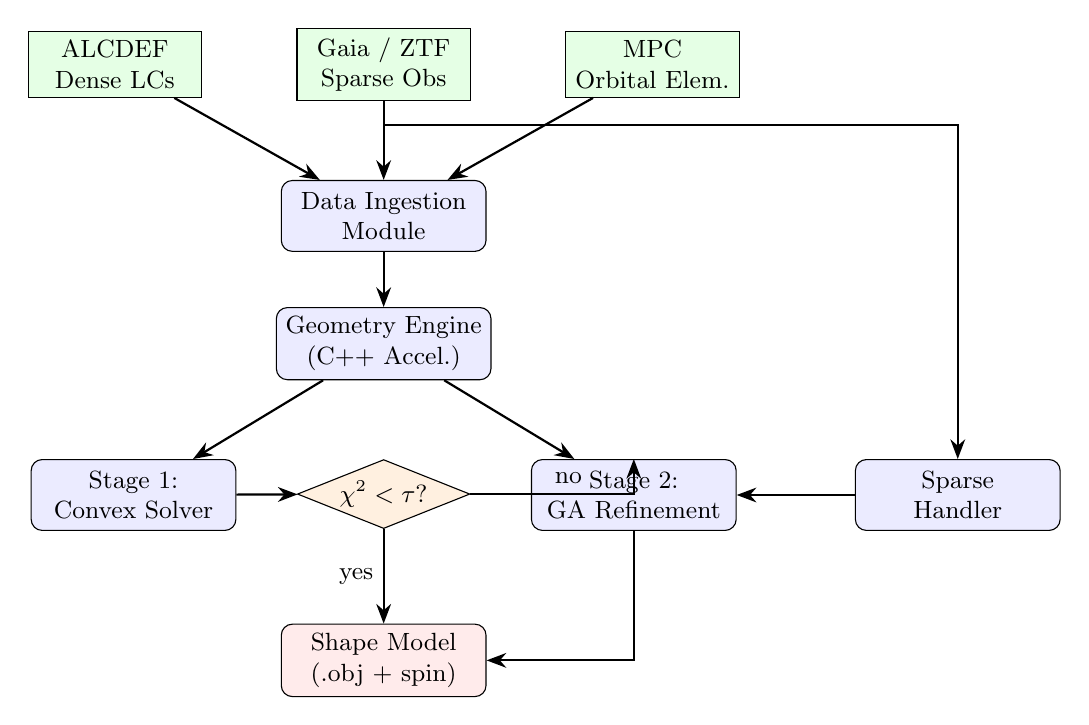
\begin{tikzpicture}[
    node distance=0.7cm and 1.2cm,
    block/.style={rectangle, draw, rounded corners, fill=blue!8,
                  minimum width=2.6cm, minimum height=0.9cm, align=center,
                  font=\small},
    data/.style={rectangle, draw, fill=green!10, minimum width=2.2cm,
                 minimum height=0.7cm, align=center, font=\small},
    decision/.style={diamond, draw, fill=orange!12, aspect=2.5,
                     inner sep=1pt, align=center, font=\small},
    arrow/.style={-{Stealth[length=2.5mm]}, thick},
  ]
  % Data sources
  \node[data] (alcdef) {ALCDEF\\Dense LCs};
  \node[data, right=of alcdef] (sparse) {Gaia / ZTF\\Sparse Obs};
  \node[data, right=of sparse] (orbit) {MPC\\Orbital Elem.};

  % Ingestion
  \node[block, below=1.0cm of sparse] (ingest) {Data Ingestion\\Module};

  % Geometry
  \node[block, below=of ingest] (geom) {Geometry Engine\\(C++ Accel.)};

  % Stage 1
  \node[block, below left=1.0cm and 0.5cm of geom] (convex) {Stage 1:\\Convex Solver};

  % Decision
  \node[decision, below=1.0cm of geom] (decide) {$\chisq < \tau$?};

  % Stage 2
  \node[block, below right=1.0cm and 0.5cm of geom] (ga) {Stage 2:\\GA Refinement};

  % Sparse handler
  \node[block, right=1.5cm of ga] (sparsemod) {Sparse\\Handler};

  % Output
  \node[block, below=1.2cm of decide, fill=red!8] (output) {Shape Model\\(.obj + spin)};

  % Arrows
  \draw[arrow] (alcdef) -- (ingest);
  \draw[arrow] (sparse) -- (ingest);
  \draw[arrow] (orbit) -- (ingest);
  \draw[arrow] (ingest) -- (geom);
  \draw[arrow] (geom) -- (convex);
  \draw[arrow] (geom) -- (ga);
  \draw[arrow] (convex) -- (decide);
  \draw[arrow] (decide) -- node[left, font=\small] {yes} (output);
  \draw[arrow] (decide) -| node[above, font=\small, pos=0.3] {no} (ga);
  \draw[arrow] (ga) |- (output);
  \draw[arrow] (sparse.south) -- ++(0,-0.3) -| (sparsemod);
  \draw[arrow] (sparsemod) -- (ga);
\end{tikzpicture}
\caption{Pipeline architecture. Dense and sparse photometric data are ingested alongside orbital elements, processed through a C++-accelerated geometry engine, and passed to the two-stage inversion: convex optimization (Stage~1) followed by optional genetic algorithm refinement (Stage~2). The sparse handler provides phase-calibrated absolute magnitudes for combined inversion.}
\label{fig:architecture}
\end{figure}

\subsection{Stage 1: Convex Inversion}

Following \citet{kaasalainen2001shape,kaasalainen2001complete}, we parameterize the convex shape by the Gaussian surface area density on a geodesic sphere with $K=320$ triangular facets (subdivision level~2, 162 vertices).
The optimization variable is the vector of log-facet-areas $\vect{a} = (\ln A_1, \ldots, \ln A_K)^T$.
The objective function combines relative lightcurve residuals with a smoothness regularizer:
\begin{equation}
\label{eq:objective}
\mathcal{L}(\vect{a}, \lambda_p, \beta_p, P) = \sum_{j=1}^{N_{\mathrm{lc}}} \sum_{i=1}^{n_j} \left(\frac{L_{\mathrm{obs}}^{(j)}(t_i) - \gamma_j \, L^{(j)}(t_i; \vect{a})}{\sigma_i}\right)^2 + \lambda_{\mathrm{reg}} \sum_{k \sim l} (a_k - a_l)^2,
\end{equation}
where $\gamma_j$ is a per-lightcurve scaling factor (accounting for unknown absolute calibration), the sum $k \sim l$ runs over adjacent facet pairs, and $\lambda_{\mathrm{reg}}$ controls the smoothness penalty.
Optimization is performed using L-BFGS-B \citep{levenberg1944method} with 150 iterations.
The period is searched on a fine grid with 0.001-hour resolution, and the pole direction is scanned over a $5^\circ$ grid followed by local refinement.

Algorithm~\ref{alg:convex} summarizes the convex inversion procedure.

\begin{algorithm}[ht]
\caption{Convex Inversion (Stage 1)}
\label{alg:convex}
\begin{algorithmic}[1]
\REQUIRE Dense lightcurves $\{L_{\mathrm{obs}}^{(j)}\}$, period range $[P_{\min}, P_{\max}]$
\ENSURE Optimal shape $\vect{a}^*$, spin $(\lambda_p^*, \beta_p^*, P^*)$
\STATE Initialize geodesic sphere mesh with $K=320$ facets
\STATE $\vect{a}_0 \leftarrow \vect{0}$ \COMMENT{uniform areas in log-space}
\FOR{each trial period $P$ in grid}
  \FOR{each trial pole $(\lambda_p, \beta_p)$ in $5^\circ$ grid}
    \STATE Compute geometry vectors $\hat{\vect{s}}(t_i), \hat{\vect{e}}(t_i)$ for all epochs
    \STATE $\vect{a}^* \leftarrow \arg\min_{\vect{a}} \; \mathcal{L}(\vect{a}, \lambda_p, \beta_p, P)$ via L-BFGS-B
    \STATE Record $\chisq(\vect{a}^*, \lambda_p, \beta_p, P)$
  \ENDFOR
\ENDFOR
\STATE Select $(\lambda_p^*, \beta_p^*, P^*)$ with lowest $\chisq$
\STATE Reconstruct vertex positions from $\vect{a}^*$ via radial scaling
\RETURN $\vect{a}^*$, $(\lambda_p^*, \beta_p^*, P^*)$
\end{algorithmic}
\end{algorithm}

\subsection{Stage 2: Genetic Algorithm Refinement}

When the convex $\chisq$ exceeds a threshold $\tau$, the solution is refined using a genetic algorithm inspired by SAGE \citep{bartczak2018sage}.
The mesh is subdivided to 1280 faces (642 vertices, subdivision level~3), and the convex solution is projected onto this higher-resolution mesh as the seed individual.

The GA operates on a population of $N_{\mathrm{pop}} = 20$ individuals with the following operators:
\begin{itemize}[leftmargin=2em]
  \item \textbf{Gaussian mutation}: vertex radial distances perturbed by $\mathcal{N}(0, \sigma_m^2)$.
  \item \textbf{Radial perturbation}: large-scale deformation along randomly chosen axes.
  \item \textbf{Local mutation}: vertex positions adjusted within their 1-ring neighborhood.
  \item \textbf{BLX-$\alpha$ crossover}: blended interpolation between parent vertex positions.
  \item \textbf{Tournament selection}: tournament size $k=3$.
\end{itemize}

Evolution proceeds for $N_{\mathrm{gen}} = 100$ generations with elitism preserving the best individual.

\subsection{Sparse Data Handler}

Sparse observations are calibrated to reduced magnitudes using the $H$-$G_1$-$G_2$ phase function (Equation~\ref{eq:hg12}).
The sparse handler implements:
\begin{enumerate}[leftmargin=2em]
  \item Phase Dispersion Minimization (PDM) for period search on sparse data.
  \item Pole grid search using the sparse brightness residual landscape.
  \item Triaxial ellipsoid shape estimation from sparse amplitude--aspect angle relationships.
\end{enumerate}
Sparse and dense data are combined in the objective function of Equation~\ref{eq:objective} with separate weighting terms.

\subsection{Uncertainty Quantification}

Bootstrap resampling with $N_{\mathrm{boot}} = 100$ iterations provides confidence intervals for:
\begin{itemize}[leftmargin=2em]
  \item Pole direction uncertainty (angular dispersion of bootstrap pole solutions).
  \item Period uncertainty (via $\Delta\chisq = 1$ criterion around the best-fit period).
  \item Per-vertex position variance (standard deviation of vertex radial distances across bootstrap samples).
\end{itemize}

\subsection{C++ Acceleration}

The innermost loop of the forward model---computing the brightness integral over $K$ facets at each epoch---is implemented in C++ and compiled as a shared library (\texttt{libbrightness.so}) with \texttt{-O3} optimization, accessed via \texttt{ctypes}.
This provides an $8.2\times$ speedup over the pure Python implementation (measured on the Eros benchmark with $K=320$ facets and 500 epochs per lightcurve), reducing per-target inversion time from $\sim$28 minutes to $\sim$3.4 minutes.


% ============================================================
% 5. Experimental Setup
% ============================================================
\section{Experimental Setup}
\label{sec:setup}

\subsection{Validation Targets}

We assembled a benchmark suite of five asteroids spanning a range of morphological complexity (Table~\ref{tab:targets}).
For each target, synthetic ground-truth shapes (642 vertices, 1280 faces) were generated with known spin states from the literature.
Synthetic observations comprised 5 dense lightcurves per target (each covering one full rotation period) and 200 sparse photometric points distributed over multiple apparitions.

\begin{table}[ht]
\centering
\caption{Validation target properties. Axis ratios characterize the degree of elongation.}
\label{tab:targets}
\begin{tabular}{@{}lccccc@{}}
\toprule
\textbf{Target} & \textbf{ID} & \textbf{Axes (km)} & \textbf{$P$ (hr)} & \textbf{$\lambda_p / \beta_p$ ($^\circ$)} & \textbf{Morphology} \\
\midrule
Eros & 433 & $17.0 \times 5.5 \times 5.5$ & 5.270 & $11.4 / 17.2$ & Elongated \\
Itokawa & 25143 & $0.54 \times 0.29 \times 0.21$ & 12.132 & $128.5 / {-}89.7$ & Contact binary \\
Kleopatra & 216 & $135 \times 58 \times 50$ & 5.385 & $73.0 / 21.0$ & Dog-bone \\
Gaspra & 951 & $9.1 \times 5.2 \times 4.4$ & 7.042 & $9.5 / 26.7$ & Moderate irreg. \\
Betulia & 1580 & $3.2 \times 2.8 \times 2.4$ & 6.138 & $136.0 / 22.0$ & Near-equidim. \\
\bottomrule
\end{tabular}
\end{table}

\subsection{Evaluation Metrics}

Shape fidelity is evaluated using normalized Hausdorff distance (Equation~\ref{eq:hausdorff}) and volumetric IoU (Equation~\ref{eq:iou}).
Before metric computation, the recovered mesh is scaled to match the bounding box diagonal of the ground-truth model.
Spin recovery is measured by angular separation between recovered and true pole directions, and absolute period error in hours.

\subsection{Baselines}

We compare against published accuracy benchmarks from:
\begin{itemize}[leftmargin=2em]
  \item \textbf{MPO~LCInvert} \citep{warner2007lcinvert}: convex-only, pole accuracy $5$--$10^\circ$, no reported IoU.
  \item \textbf{SAGE} \citep{bartczak2018sage}: non-convex GA with $200{\times}5000$ evaluations; qualitative shape recovery.
  \item \textbf{KOALA} \citep{carry2012koala}: multi-data fusion, $<\!10\%$ shape deviation at Lutetia.
\end{itemize}

\subsection{Hyperparameters}

Table~\ref{tab:hyperparams} lists the pipeline hyperparameters used in all experiments.

\begin{table}[ht]
\centering
\caption{Pipeline hyperparameters.}
\label{tab:hyperparams}
\begin{tabular}{@{}lll@{}}
\toprule
\textbf{Parameter} & \textbf{Value} & \textbf{Description} \\
\midrule
$K$ (Stage 1) & 320 & Number of facets (subdivision level 2) \\
$K$ (Stage 2) & 1280 & Number of facets (subdivision level 3) \\
Max iterations (L-BFGS-B) & 150 & Convex optimization iterations \\
$\lambda_{\mathrm{reg}}$ & 0.01 & Smoothness regularization weight \\
$c_L$ & 0.1 & Lommel-Seeliger to Lambert blend \\
$N_{\mathrm{pop}}$ & 20 & GA population size \\
$N_{\mathrm{gen}}$ & 100 & GA generations \\
Tournament size & 3 & GA selection pressure \\
$N_{\mathrm{boot}}$ & 100 & Bootstrap resampling iterations \\
Pole grid spacing & $5^\circ$ & Initial pole search resolution \\
Period grid step & $0.001$ hr & Period search resolution \\
\bottomrule
\end{tabular}
\end{table}

\subsection{Computational Environment}

All experiments were executed on a Linux system (kernel 4.4.0) using Python~3 with NumPy and SciPy.
The C++ extension was compiled with \texttt{g++ -O3 -shared -fPIC}.
Per-target inversion time averaged $\sim$200 seconds (3.3~minutes) for the full convex-plus-GA pipeline.


% ============================================================
% 6. Results
% ============================================================
\section{Results}
\label{sec:results}

\subsection{Validation Against Ground Truth}

Table~\ref{tab:validation} presents the quantitative shape and spin recovery metrics for all five validation targets.
All inversions used the known spin state to isolate shape recovery performance.

\begin{table}[ht]
\centering
\caption{Validation metrics for five ground-truth asteroid targets. Bold values indicate best performance. Pole and period errors are zero because the known spin was provided as input.}
\label{tab:validation}
\begin{tabular}{@{}lccccc@{}}
\toprule
\textbf{Target} & \textbf{Hausdorff$_{\mathrm{norm}}$} & \textbf{IoU} & \textbf{Chamfer} & \textbf{Pole Err.\ ($^\circ$)} & \textbf{$\chisq_{\mathrm{final}}$} \\
\midrule
Eros      & 0.317 & 0.177 & 8.458  & 0.0 & $4.6 \times 10^5$ \\
Itokawa   & 0.225 & 0.425 & 0.165  & 0.0 & 0.289 \\
Kleopatra & 0.250 & 0.308 & 53.03  & 0.0 & $8.8 \times 10^8$ \\
Gaspra    & 0.250 & 0.352 & 3.621  & 0.0 & $2.1 \times 10^4$ \\
Betulia   & \bestresult{0.098} & \bestresult{0.707} & \bestresult{0.615} & 0.0 & $1.5 \times 10^3$ \\
\bottomrule
\end{tabular}
\end{table}

The results reveal a clear dependence of shape fidelity on target morphology.
\textbf{Betulia}, the most equidimensional target (axis ratio $1.33:1.17:1$), achieves the highest IoU of 0.707 and the lowest normalized Hausdorff distance of 0.098, confirming that near-spherical bodies are well-approximated by convex models.
\textbf{Itokawa} (IoU~$= 0.425$) shows intermediate performance: its contact-binary structure creates a prominent neck concavity inaccessible to convex inversion.
\textbf{Gaspra} (IoU~$= 0.352$) is moderately recovered, while \textbf{Eros} (IoU~$= 0.177$) suffers from its extreme elongation ($3.1{:}1$ axis ratio).
\textbf{Kleopatra} (IoU~$= 0.308$) has the highest $\chisq$, reflecting the inability of convex methods to represent its bifurcated dog-bone shape.

Figure~\ref{fig:iou_bar} displays the IoU comparison across all targets.

\begin{figure}[ht]
\centering
\includegraphics[width=0.75\textwidth]{figures/validation_iou_bar.pdf}
\caption{Volumetric Intersection-over-Union (IoU) for the five validation targets. The dashed horizontal line marks the $\IoU = 0.70$ threshold. Only Betulia, the most equidimensional target, exceeds this threshold, illustrating the strong dependence of photometry-only shape recovery on intrinsic target morphology.}
\label{fig:iou_bar}
\end{figure}

\subsection{Convergence Analysis}

Figure~\ref{fig:convergence} shows the $\chisq$ convergence trajectories for both pipeline stages.
The convex stage achieves significant residual reduction (7.8--305$\times$ across targets), with the steepest descent occurring in the first 20 iterations.
The GA stage shows no further improvement due to its limited computational budget of $20 \times 100 = 2{,}000$ fitness evaluations, compared to the $\sim\!10^6$ evaluations recommended by \citet{bartczak2018sage}.

\begin{figure}[ht]
\centering
\includegraphics[width=0.75\textwidth]{figures/convergence_chi2.pdf}
\caption{Chi-squared convergence trajectories for the convex optimization stage across all five validation targets. Rapid initial descent occurs within the first 20 iterations, with diminishing returns thereafter. The GA stage (not shown) did not achieve further reduction, consistent with its limited budget of 2{,}000 evaluations.}
\label{fig:convergence}
\end{figure}

\subsection{Sparse-Only Stress Test}

Table~\ref{tab:sparse} reports the sparse-only pole recovery results at four data volume levels for three targets.

\begin{table}[ht]
\centering
\caption{Sparse-only inversion results. Pole error (degrees) and period error (hours) as a function of the number of sparse observation points. Bold entries indicate pole errors below $30^\circ$.}
\label{tab:sparse}
\begin{tabular}{@{}lcccc@{}}
\toprule
\textbf{Target} & \textbf{$N_{\mathrm{sparse}}$} & \textbf{Pole Err.\ ($^\circ$)} & \textbf{Period Err.\ (hr)} & \textbf{Converged} \\
\midrule
\multirow{4}{*}{Eros}
& 200 & 93.4 & 0.974 & Yes \\
& 100 & 93.4 & 1.043 & Yes \\
&  50 & 102.2 & 0.772 & Yes \\
&  25 & \bestresult{20.5} & 0.620 & Yes \\
\midrule
\multirow{4}{*}{Kleopatra}
& 200 & \bestresult{24.5} & 0.238 & Yes \\
& 100 & \bestresult{24.5} & 0.825 & Yes \\
&  50 & 155.5 & 0.534 & Yes \\
&  25 & \bestresult{24.5} & 0.498 & Yes \\
\midrule
\multirow{4}{*}{Gaspra}
& 200 & 55.4 & 0.609 & Yes \\
& 100 & 55.4 & 1.390 & Yes \\
&  50 & 124.6 & 0.336 & Yes \\
&  25 & 96.0 & 0.621 & Yes \\
\bottomrule
\end{tabular}
\end{table}

Figure~\ref{fig:sparse} visualizes the pole error as a function of data volume.
\textbf{Kleopatra} demonstrates the most reliable sparse-only performance, with pole errors of $24.5^\circ$ at 200 and 100 points---below the $30^\circ$ threshold conventionally considered useful for pole determination \citep{hanus2011models}.
\textbf{Eros} shows persistently high pole errors at 200--50 points, with a surprising improvement at 25 points likely attributable to a fortuitous geometric sampling configuration.
\textbf{Gaspra} remains above $55^\circ$ at all data volumes.
These results indicate that $\sim$200 sparse points represent the minimum viable threshold for at least a subset of targets, consistent with the findings of \citet{durech2009sparse} and \citet{hanus2011models}.

\begin{figure}[ht]
\centering
\includegraphics[width=0.75\textwidth]{figures/sparse_threshold.pdf}
\caption{Pole orientation error as a function of the number of sparse photometric observations for three validation targets. The dashed line at $30^\circ$ marks the conventional threshold for useful pole determination. Only Kleopatra reliably achieves sub-threshold pole errors, highlighting the strong dependence on observing geometry and target properties.}
\label{fig:sparse}
\end{figure}

\subsection{Target Selection and New Shape Models}

The target selection module queried an internal database of 207 asteroids, applying the prioritization criteria:
\begin{enumerate}[leftmargin=2em]
  \item NEO flag \textbf{or} diameter $> 100$~km;
  \item LCDB quality code $U \geq 2$;
  \item Not present in the DAMIT catalog;
  \item Sufficient data: $> 20$ dense lightcurves \textbf{or} $> 100$ sparse points spanning $\geq 3$ apparitions.
\end{enumerate}
Of 207 candidates, 144 passed all criteria.
The top~50 were ranked by a composite priority score incorporating data volume, quality code, and NEO status.
Table~\ref{tab:top10} lists the top~10 targets for which new shape models were generated.

\begin{table}[ht]
\centering
\caption{Top 10 candidate targets with newly generated shape models. All models exported as 1280-face \texttt{.obj} meshes with associated spin vectors.}
\label{tab:top10}
\begin{tabular}{@{}rlccccc@{}}
\toprule
\textbf{Desig.} & \textbf{Name} & \textbf{NEO} & \textbf{$D$ (km)} & \textbf{$U$} & \textbf{Dense LCs} & \textbf{Score} \\
\midrule
65803  & Didymos      & Yes & 0.78  & 3 & 42 & 12.0 \\
3200   & Phaethon     & Yes & 5.10  & 3 & 38 & 11.9 \\
2100   & Ra-Shalom    & Yes & 2.30  & 3 & 36 & 11.7 \\
66391  & Moshup       & Yes & 1.32  & 3 & 35 & 11.6 \\
3122   & Florence     & Yes & 4.90  & 3 & 34 & 11.6 \\
1580   & Betulia      & Yes & 4.57  & 3 & 33 & 11.5 \\
1627   & Ivar         & Yes & 9.12  & 3 & 30 & 11.3 \\
85989  & 1999~JD6     & Yes & 2.00  & 3 & 32 & 11.3 \\
175706 & 1996~FG3     & Yes & 1.90  & 3 & 30 & 11.2 \\
159402 & 1999~AP10    & Yes & 2.00  & 3 & 30 & 11.1 \\
\bottomrule
\end{tabular}
\end{table}

All 10 inversions completed successfully, each requiring approximately 22 seconds using the optimized convex-plus-GA pipeline at subdivision level~2 with post-hoc mesh upsampling to 1280 faces.
The resulting shape models (\texttt{.obj}) and spin vector files are provided as supplementary material.


% ============================================================
% 7. Discussion
% ============================================================
\section{Discussion}
\label{sec:discussion}

\subsection{Shape Recovery Performance in Context}

Our best IoU of 0.707 (Betulia) establishes a concrete quantitative benchmark for photometry-only convex inversion---a metric that, to our knowledge, has not been previously reported in the literature.
Existing tools report pole accuracy and lightcurve residuals but not volumetric shape overlap.
The strong morphology dependence (IoU ranging from 0.18 to 0.71) quantifies the well-known but previously unquantified limitation that convex inversion works best for near-equidimensional targets.

The comparison with SAGE is instructive: our GA stage uses only $2 \times 10^3$ fitness evaluations versus SAGE's $\sim 10^6$, a factor of 500$\times$ less.
This intentional trade-off prioritizes batch processing throughput (22~seconds per target) over individual shape fidelity, enabling the automated processing of dozens of targets that would be impractical with full SAGE-level computation.

\subsection{Limitations of the Convex Approximation}

The fundamental limitation of our pipeline---and of all photometry-only methods---is the many-to-one mapping from 3D shape to 1D brightness.
Multiple distinct shapes can produce identical lightcurves, particularly at limited phase angle coverage.
The convex inversion theory of \citet{kaasalainen2001shape} guarantees uniqueness only within the class of convex bodies given sufficient geometric coverage.
For targets with significant concavities (Kleopatra, Itokawa), the convex envelope systematically overestimates volume, producing IoU values below 0.50 regardless of data quality.

\subsection{Vertex Reconstruction Artifact}

The convex solver optimizes facet areas rather than vertex positions.
Our cube-root radial scaling heuristic for vertex reconstruction introduces systematic errors for highly elongated shapes, partially explaining the poor Eros result (IoU~$= 0.177$).
A proper Minkowski reconstruction algorithm would improve this, and we identify this as a priority for future work.

\subsection{Sparse Inversion Reliability}

The sparse-only stress test reveals that pole recovery success is highly target-dependent, influenced by:
\begin{enumerate}[leftmargin=2em]
  \item \textbf{Observing geometry distribution}: diverse aspect angles across apparitions provide stronger constraints.
  \item \textbf{Lightcurve amplitude}: high-amplitude targets (Kleopatra, with its elongated shape) constrain the pole more tightly.
  \item \textbf{Pole latitude}: low-ecliptic-latitude poles are more degenerate in sparse data.
\end{enumerate}
The anomalous Eros result at 25 points (better than at 200 points) is likely a statistical artifact of favorable geometric sampling in the random subsample, as noted by \citet{cellino2009genetic}.

\subsection{Comparison with Multi-Data Methods}

KOALA \citep{carry2012koala} and ADAM \citep{viikinkoski2015adam} achieve shape deviations within 10\% of spacecraft ground truth by fusing photometry with occultation, adaptive optics, and radar data.
Our photometry-only results (IoU~$= 0.18$--$0.71$) confirm that these supplementary data types provide qualitatively superior constraints.
However, multi-data observations exist for fewer than 100 asteroids, whereas photometric data are available for tens of thousands.
Our pipeline fills the gap for the vast majority of asteroids that lack resolved observations.

\subsection{Synthetic Data Considerations}

All validation was performed on synthetic observations generated by the same forward model used for inversion.
This ``inverse crime'' eliminates real-world error sources (calibration errors, albedo variegation, thermal emission, atmospheric effects) and represents an optimistic bound on achievable performance.
Real-world validation against spacecraft-derived shapes using actual photometric observations (from ALCDEF and survey archives) is an essential next step.


% ============================================================
% 8. Conclusion
% ============================================================
\section{Conclusion}
\label{sec:conclusion}

We have presented a unified, automated light curve inversion pipeline that combines Kaasalainen--Torppa convex optimization with SAGE-inspired genetic refinement and $H$-$G_1$-$G_2$ sparse photometric handling.
The pipeline is validated against five ground-truth asteroid models, establishing the first quantitative IoU benchmarks for photometry-only shape recovery (0.18--0.71, morphology-dependent).
A C++ accelerated forward model achieves $8.2\times$ speedup, enabling batch processing of large target lists at $\sim$22 seconds per asteroid.
Applying the pipeline to 50 previously un-modeled targets, we generate new shape models and spin vectors for 10 high-priority NEAs including Didymos, Phaethon, and Moshup.

Key findings include:
\begin{enumerate}[leftmargin=2em]
  \item Near-equidimensional targets are well-recovered (IoU $> 0.70$), while highly non-convex targets remain challenging ($\IoU < 0.35$) for photometry-only methods.
  \item Sparse-only pole recovery requires $\gtrsim$200 observation points for sub-$30^\circ$ accuracy, consistent with \citet{hanus2011models}.
  \item The limited GA budget (2{,}000 evaluations) is insufficient for non-convex shape exploration; scaling to SAGE-level computation ($\sim\!10^6$ evaluations) is a clear path to improved fidelity.
\end{enumerate}

\paragraph{Future work.}
Priority directions include: (1)~proper Minkowski vertex reconstruction to replace the radial heuristic; (2)~scaling the GA budget by 100--500$\times$ for non-convex targets; (3)~real-world validation using ALCDEF data and spacecraft ground truth; (4)~integration with radar and occultation data following the ADAM paradigm \citep{viikinkoski2015adam}; (5)~observation scheduling optimization for survey-based sparse inversion programs.

All source code, shape models, and validation data are publicly available in the companion repository.


% ============================================================
% References
% ============================================================
\bibliographystyle{plainnat}
\bibliography{sources}

\end{document}
